\chapter{Avaliação} \label{ch:evaluation}

Este Capítulo apresenta resultados comparativos da solução desenvolvida com a 
aplicação original. A Seção \ref{sect:methodology} apresenta detalhes da 
metodologia de avaliação e a Seção \ref{sect:results} disserta sobre os 
resultados.


\section{Metodologia de Avaliação} \label{sect:methodology}

Os experimentos foram realizados no Parque Computacional de Alto Desempenho 
(PCAD) da UFRGS. Eles ocorreram nos nós de computação draco, sua 
configuração é mostrada na Tabela \ref{tab:draco_config}.

\begin{table}[H]
\centering
\begin{tabular}{l l} \toprule
\textbf{Parâmetro}  &  \textbf{Configuração} \\ 
\midrule
Processador     & 2 x Intel Xeon E5-2630 (Q1'12) Sandy Bridge, 2,5 GHz  
\\
Número de Núcleos    & 16 núcleos (8 por CPU)  \\
Memória       & 64 GB DDR3 RAM   \\
\end{tabular}
\caption{Configurações dos nós draco.}
\label{tab:draco_config}
\end{table}


A Figura \ref{fig:experiment_arch} exibe a arquitetura que foi seguida durante 
os experimentos. Como os experimentos com o Spark acessam dados direto do HDFS, 
primeiramente executamos o Hadoop. Um dos nós era responsável por executar o 
\emph{namenode} e também executava uma instância de \emph{datanode}. Os demais 
executavam apenas instâncias de \emph{datanodes}.


\begin{figure}[ht]
\centerline{
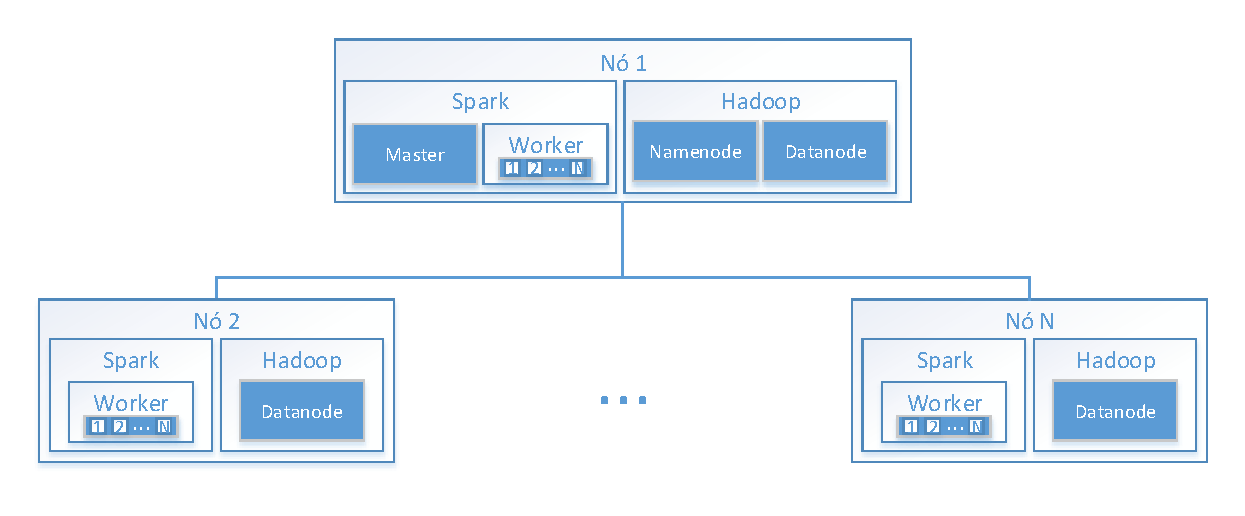
\includegraphics[width=0.9\textwidth]{./img/experiments_arch.pdf}}
 \caption{Arquitetura de aplicações durante os experimentos.}
 \label{fig:experiment_arch}
\end{figure}


O gerenciador de cluster utilizado foi o do próprio Spark ao invés do YARN. 
Essa decisão foi tomada durante os testes pois seus logs mostraram 
informações mais claras sobre o que estava ocorrendo. A instânciação dele foi 
similar àquela utilizada no Hadoop, um nó executou como \emph{mestre} e 
\emph{trabalhador} enquanto os demais executaram apenas como 
\emph{trabalhadores}. 

Cada \emph{trabalhador} do Spark instancia N \emph{executores}, responsáveis 
por processar tarefas. Cada um destes possui uma quantidade de cores e uma 
quantidade de memória dedicada. Durante os experimentos, parametrizamos a 
\emph{Engine} para que cada \emph{trabalhador} instanciasse 15 
\emph{executores}, cada um com 2 cores e 4 GB de memória para processamento de 
tarefas.

Realizamos testes com um nó, utilizando a aplicação original, um, dois e três 
nós, utilizando a aplicação modificada. Cada teste foi executado 
aproximadamente 30 vezes (a salvo algum problema de execução em alguma 
repetição) para garantir a confiabilidade de seus resultados. 


\section{Experimentos e Resultados} \label{sect:results}

A carga de trabalho dos experimentos já no formato CSV (entrada para a fase de 
pré-processamento no StarVZ), tinha um somatório de 12 GB. Ela consiste em 
rastros de execução de uma aplicação cholesky e foi escolhida pois era a maior
entrada que tínhamos no momento. O tamanho de cada um dos arquivos pode ser 
visualizado na Tabela \ref{tab:input_sz}.

\begin{table}[H]
\centering
\begin{tabular}{l c} \toprule
\textbf{Arquivo}  &  \textbf{Tamanho} \\ 
\midrule
state.csv	& 6.8 GB \\
variables.csv  	& 2.5 GB \\
link.csv       	& 304 MB \\
dag.csv        	& 270 MB \\
entities.csv	& 73 KB \\
events.csv	& 1.8 GB \\
\textbf{Total}  & 12 GB  \\
\end{tabular}
\caption{Detalhamento da carga de trabalho.}
\label{tab:input_sz}
\end{table}

Durante a implementação, optou-se por manter o processamento do arquivo entities 
no formato sequencial pois esse arquivo armazena apenas informações de 
plataforma e por isso, costuma não passar da ordem de tamanho de KB. Podemos 
observar que isso se confirma nesta carga de trabalho.


Foram executadas 30 repetições em cada teste, todavia, os experimentos com o 
Spark apresentaram problemas em algumas execuções. Com um nó, 3 execuções foram 
interrompidas e com dois e três nós, uma. Nesses casos, consideramos apenas 
aquelas que processaram com sucesso (27, 29 e 29 repetições, respectivamente). 

A Figura \ref{fig:total_full} mostra a média do tempo total de execução dos 
experimentos e o desvio padrão no topo da barra, em função do nível de 
paralelismo (quantidade de executores de tarefas) em cada nó. A execução 
original, de forma sequencial, levou em média, 1489,02 segundos para completar 
o processamento. Já as execuções com a aplicação adaptada para utilizar o 
Spark, com apenas um nó levou em média 708,17 segundos, com dois, 460,81 
segundos e com três, 385,44 segundos. Isso consiste em um \emph{speedup} de 
respectivamente 2,10x, 3,23x e 3,86x em relação ao original.

\begin{figure}[ht]
\centerline{
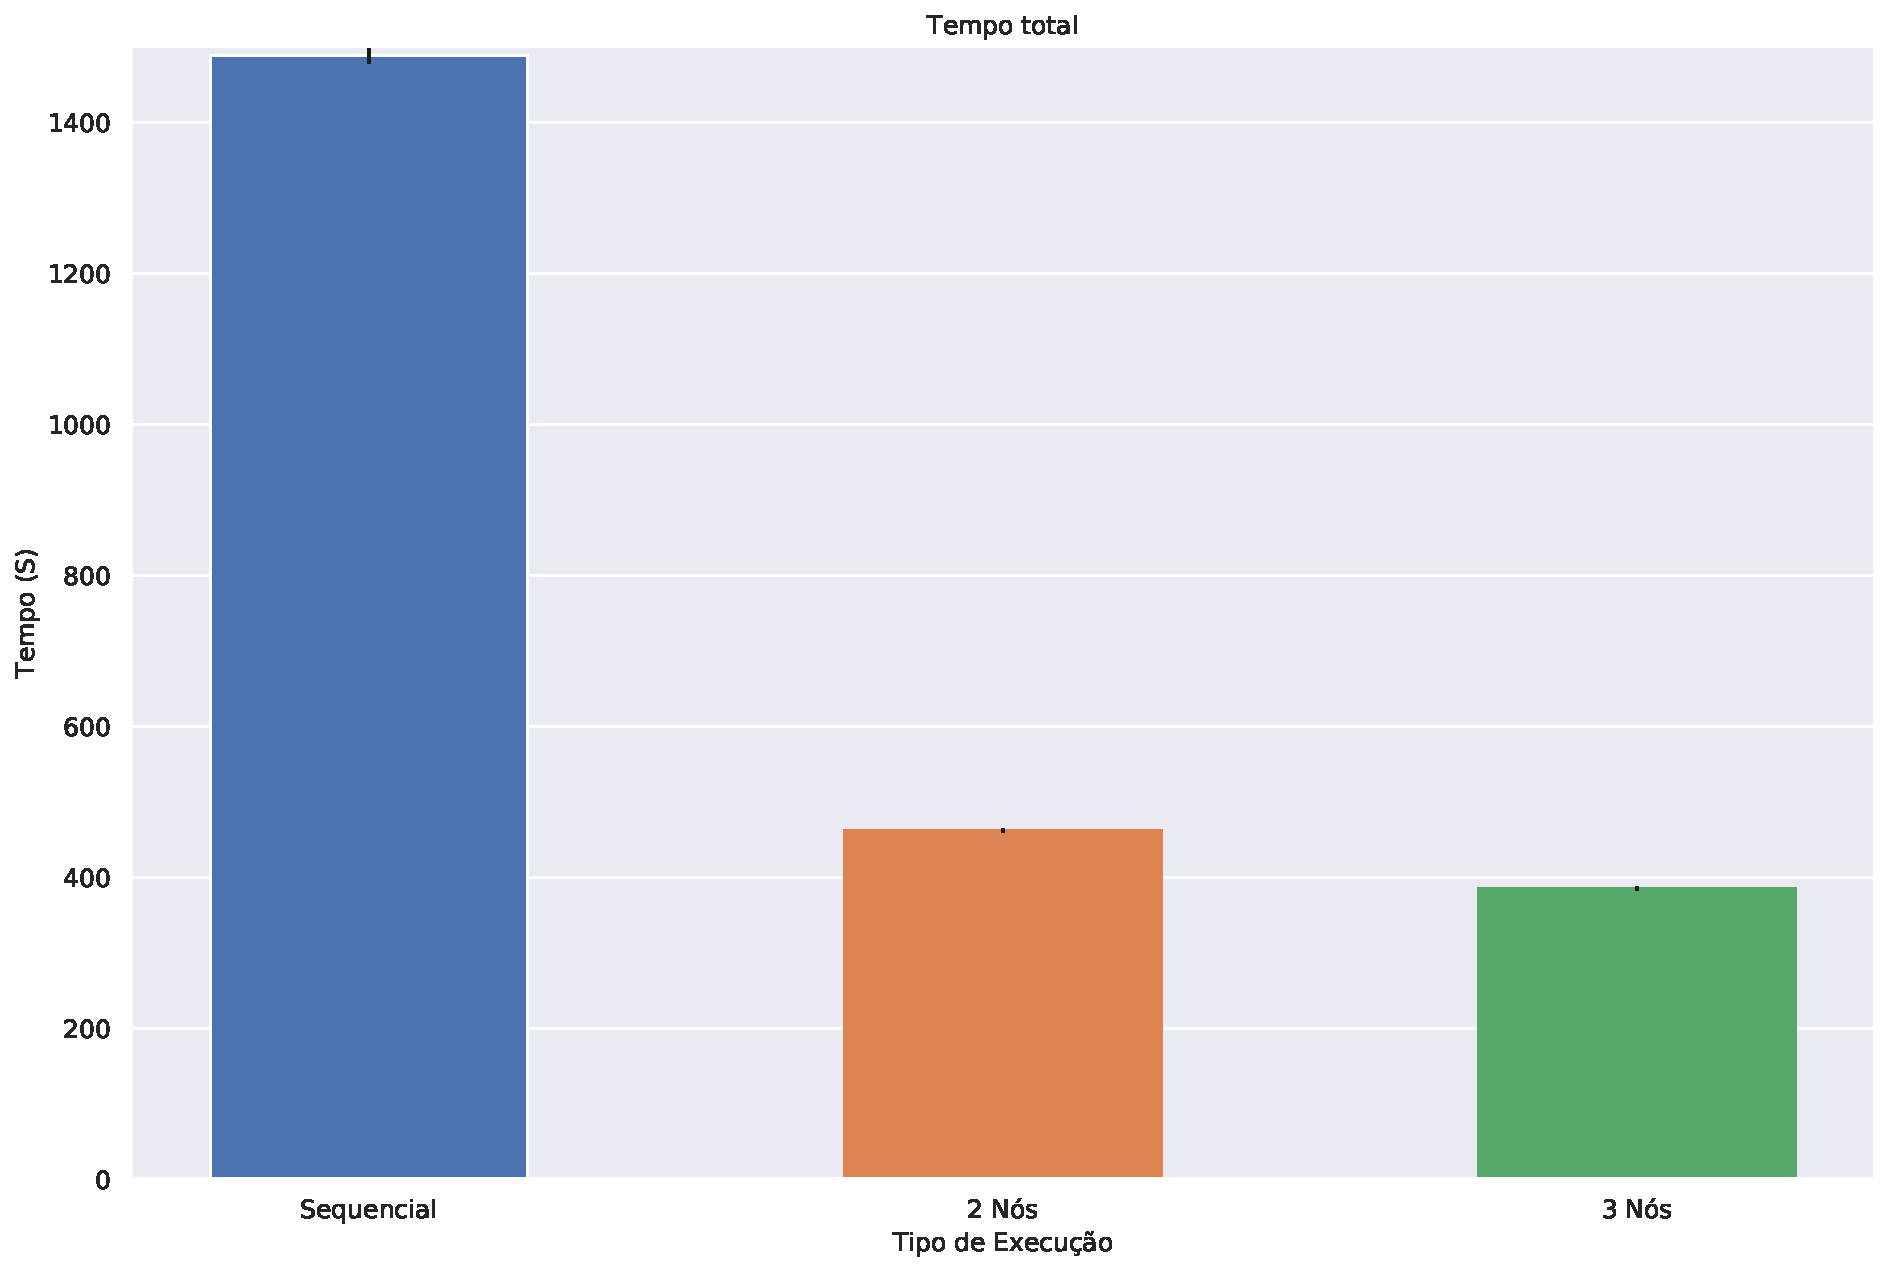
\includegraphics[width=0.9\textwidth]{./img/total.pdf}}
 \caption{Tempo total de execução da aplicação.}
 \label{fig:total_full}
\end{figure}


Segmentamos a análise pelas etapas exibidas na Figura 
\ref{fig:spark-starvz-flow}, seus tempos de execução podem ser visualizados na 
Figura \ref{fig:total_step}. Analisando os resultados e o código, identificamos 
quatro grupos de manipulações.

O primeiro e mais trivial deles, é o grupo em que observa-se quase nenhuma 
variação, pois não existe motivo para ela ocorrer. É o caso do tratamento de 
Entities, que manteve-se praticamente o mesmo e isso é observado em seus tempos 
de execução, que pode ser visto com mais detalhes na Tabela 


Fica claro que o processamento dominante em todos 
os tipos de execução é o de State. Isso é causado por uma associação entre seu 
tamanho, pois esta tabela é gerada pelo maior arquivo, além das manipulações 
realizadas em sua etapa de tratamento, que disparam jobs Spark e comunicação 
entre executores. 





\begin{figure}[H]
\centerline{
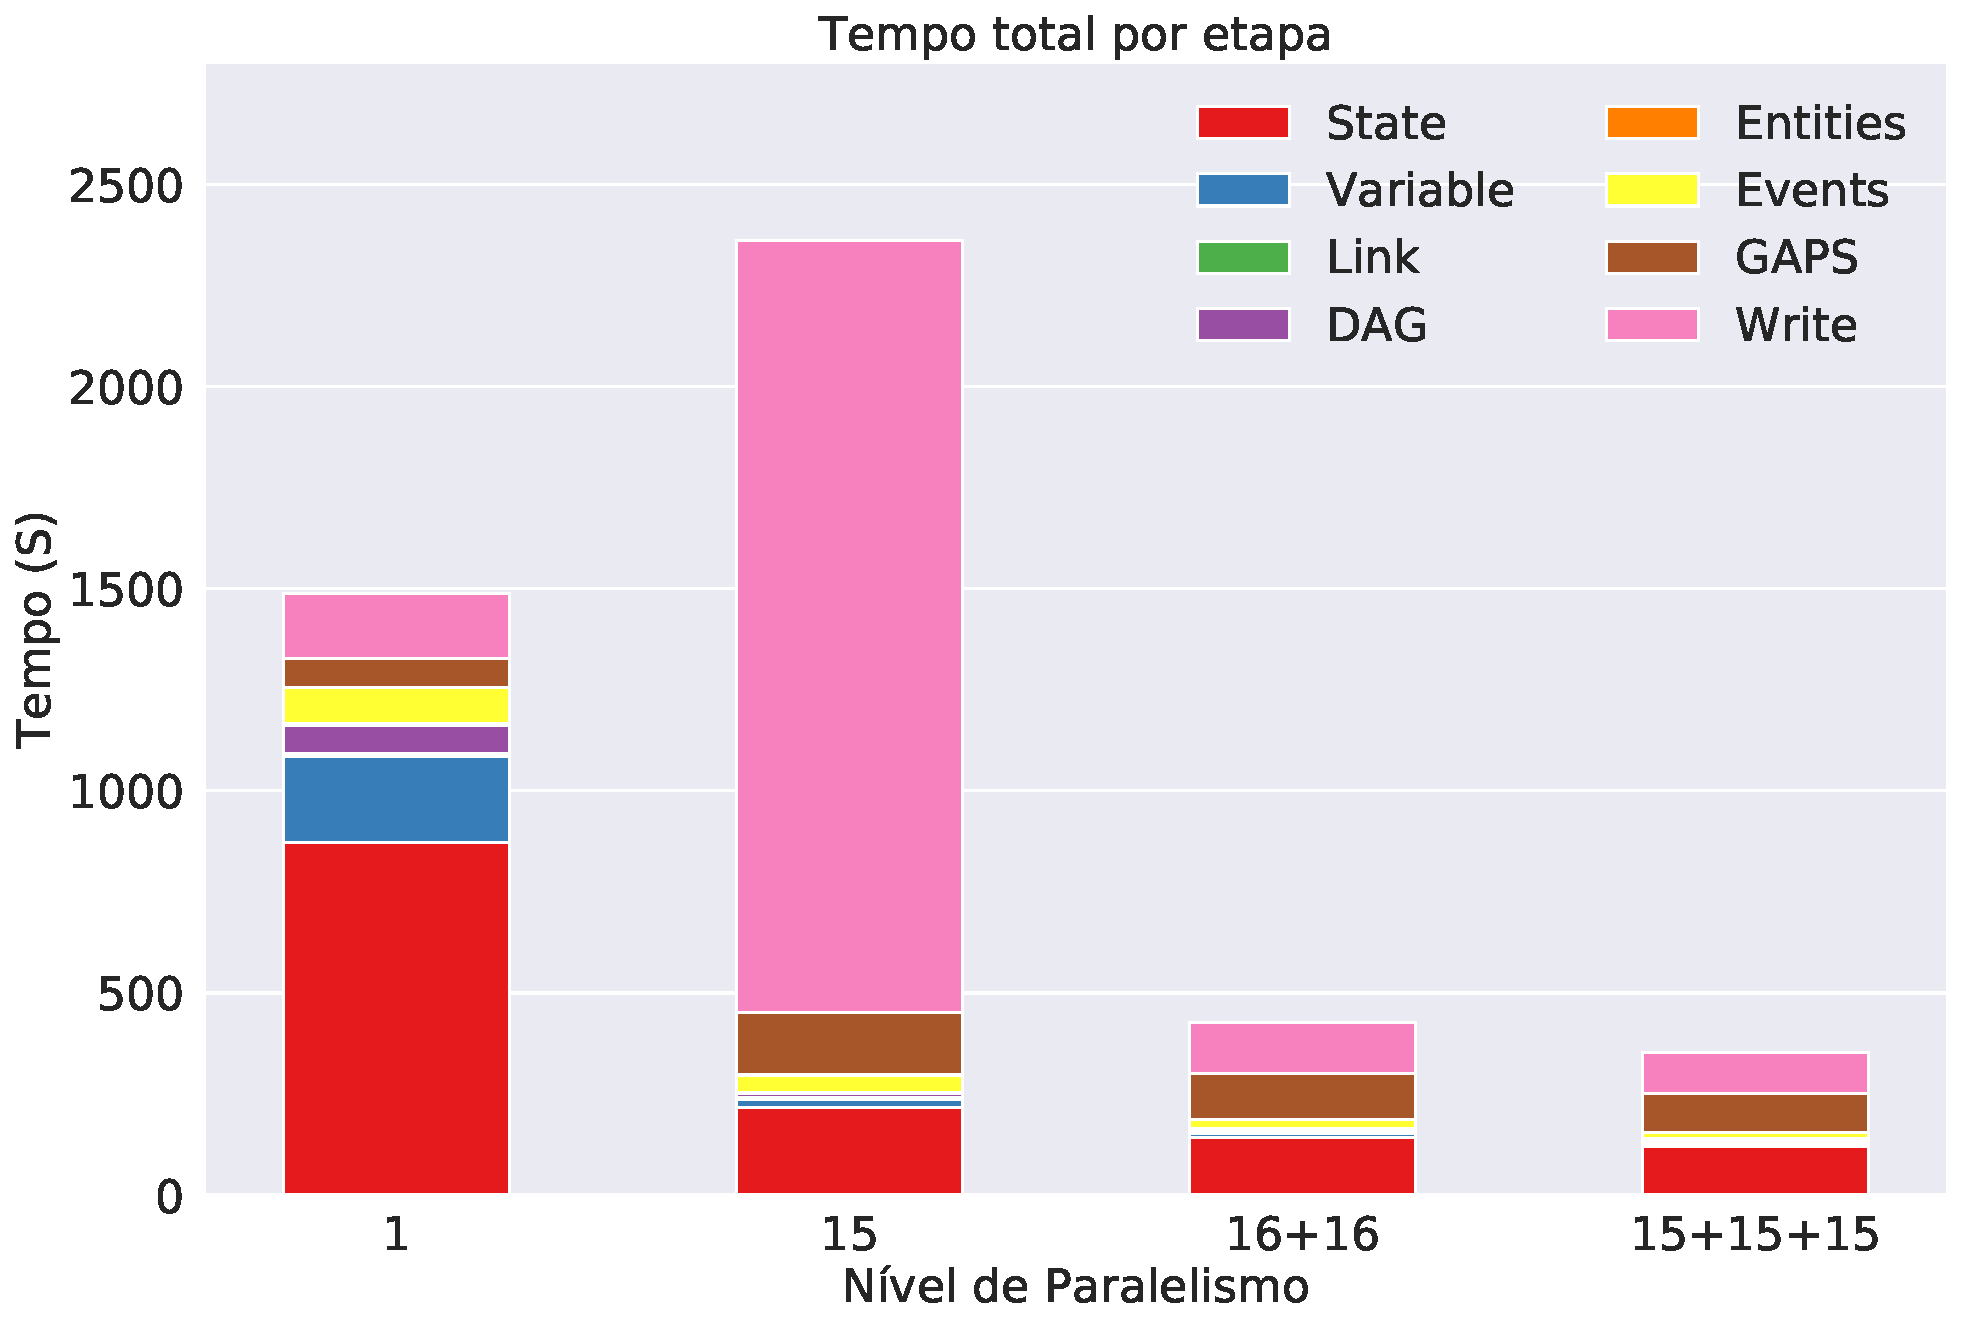
\includegraphics[width=0.5\textwidth]{./img/total_step.pdf}}
 \caption{Tempos de execução segmentados por etapas.}
 \label{fig:total_step}
\end{figure}

Analisando o processamento de Variables, o segundo maior arquivo da carga de 
trabalho, na execução sequencial é o segundo mais custoso levando em média 
210,77 segundos. Já com o Spark. seu tempo cai para 21,17 segundos com 1 nó, 
10,44 segundos com 2 nós e 7,50 segundos com três. Essa grande redução de 
tempo está associada as otimizações realizadas pela Engine, tendo em vista que 
essa tabela é apenas filtrada, apenas os dados necessários são carregados para 
a memória durante essa etapa. É importante salientar que uma parte dessas 
economias serão penalizadas quando essa tabela for necessária por completo, 
para uma junção ou até mesmo para a escrita, embora a \emph{Engine} consiga 
otimizar bastante carregando apenas os dados filtrados para memória.

Os processamentos de Link e de DAG são similares ao de Variables. Não há ações 
que precisem com que a \emph{Engine} traga muitos dados para a memória e, 
portanto, observamos melhora no desempenho. A média dos tempos de execução, na 
ordem da esquerda para a direita no gráfico para Link são de, em segundos, 
8,93, 4,59, 3,84 e 3,53. Para DAG esses valores são de 69,14, 10,10, 7,58 e 
6,76.

O processamento de entities foi mantido na forma sequencial devido ao seu 
tamanho ser na ordem de KB. Seu tempo de processamento tem um valor irrisório 
a ponto de ser difícil de observar no gráfico. Em média, para a execução com a 
aplicação no modo sequencial ele levou 3,07 segundos, já com o Spark, com 
um, dois e três nós foram respectivamente 2,42, 2,29 e 2,30 segundos. Portanto, 
essa decisão teve pouco impacto no resultado final, o que era o objetivo já que 
sua constribuição para o tempo total da aplicação é tão pequeno.

O cálculo de GAPS foi levantado durante a implementação como um ponto de 
atenção, devido ao seu tempo ter aumentado de forma considerável em experimentos 
locais. Olhando para os tempos de execução temos, em segundos, 71,51 na 
execução sequencial, 154,03 na execução com 1 nó utilizando Spark, 110,83 na 
execução com 2 nós e 95,22 utilizando 3 nós. Esse processamento utiliza duas 
funções recursivas e, dentro de rodada de iteração, é realizada uma junção. 
Estas operações são custosas, principalmente quando realizadas em tabelas 
grandes pois o Spark irá realizar um \emph{shuffle join} 
\cite{ref:sparkbook}. Nesse tipo de junção, cada nó precisa falar com cada nó, 
sendo um gargalo para o processamento como um todo. Dentro desse processamento 
há ainda a junção de uma tabela derivada de state que, conforme mencionado 
anteriormente, é a maior tabela que temos, exigindo que muitos dados sejam 
carregados para a memória.

A escrita se beneficiou da execução distribuída, obtivemos em média os 
tempos de 162,19 segundos para a sequencial, 125,6 segundos (\textit{speedup} 
de 1,29 em relação a primeira) para a distribuída com dois nós e 102,87 
segundos (\textit{speedup} de 1,57 em relação a primeira) para três. 
Inicialmente, esperávamos um ganho de desempenho um pouco melhor, todavia, 
algumas operações de filtragem só são executadas nesse momento (execução 
\textit{lazy} da engine), o que justifica o ganho inferior ao esperado.


